\documentclass[12pt,reqno]{report}
\usepackage{amsfonts}
\usepackage{stmaryrd}
\usepackage[UTF8]{ctex}
\usepackage{xeCJK} % 添加 xeCJK 宏包以使用中文数字
\usepackage{fontspec} 
\usepackage{mathtools}
\usepackage{setspace}
\usepackage{float}
\usepackage{subfigure}
\usepackage[ruled,linesnumbered,lined,boxed,commentsnumbered]{algorithm2e}
\usepackage{geometry}
\geometry{a4paper, total={170mm,257mm}, left=20mm, top=20mm}
\usepackage{graphicx,cases}
\usepackage{xcolor}
\usepackage{sectsty}
\usepackage{braket}
\usepackage{amsmath, amssymb, mathrsfs, amsthm}
\usepackage{hyperref}
\usepackage{cleveref}
\usepackage{xpatch}
\usepackage[backend=biber, style=numeric, sorting=none]{biblatex}
\addbibresource{refer.bib} % 指定引用的.bib文件
\usepackage{fancyhdr}

% 自定义章节标题格式
\usepackage{titlesec}
\titleformat{\chapter}{\centering\normalfont\huge\bfseries}{第\ \thechapter\ 章}{20pt}{\huge}
\titleformat{\section}{\centering\normalfont\Large\bfseries}{\thechapter.\thesection}{1em}{\Large}
\titleformat{\subsection}{\normalfont\large\bfseries}{\thechapter.\thesubsection}{1em}
{}
\renewcommand\thechapter{\arabic{chapter}} % 设置章标题为中文数字
\renewcommand\thesection{\arabic{section}} % 设置章标题为阿拉伯数字
\newcounter{romanpage}

% 定义定理环境
\newtheorem{theorem}{\hspace{2em} 定理}[section] 
\newtheorem{definition}[theorem]{\hspace{2em} 定义}
\newtheorem{lemma}[theorem]{\hspace{2em} 引理} 
\newtheorem{corollary}[theorem]{\hspace{2em} 推论} 
\newtheorem{example}[theorem]{\hspace{2em} 例}
\newtheorem{property}{\hspace{2em} 性质}
%把定理后面的点去掉
\makeatletter
\AtBeginDocument{\xpatchcmd{\cref@thmoptarg}{\thm@headpunct{.}}{\thm@headpunct{}}{}{}}
\AtBeginDocument{\xpatchcmd{\cref@thmnoarg}{\thm@headpunct{.}}{\thm@headpunct{}}{}{}}
\makeatother

\renewcommand{\proofname}{\bfseries\upshape 证明\nopunct}
\newcounter{methodcount}[section] % 方法环境的计数器
\newtheorem{method}[methodcount]{\hspace{2em} 方法} % 方法环境的样式
\renewcommand\themethodcount{\chinese{methodcount}} % 方法环境的编号格式
\renewcommand\theexample{\arabic{section}.\arabic{example}}
\renewcommand\thetheorem{\arabic{section}.\arabic{theorem}} 
\renewcommand\thedefinition{\arabic{section}.\arabic{definition}} 
\crefname{theorem}{\textbf{定理}}{定理}
\crefname{lemma}{\textbf{引理}}{引理}
\crefname{example}{\textbf{例}}{例}
\crefname{definition}{定义}{定义}
\crefname{algorithm}{算法}{算法}
\crefformat{equation}{#2(#1)式#3}

% 自定义定理样式,包括标题和后面的序号都加粗
\newtheoremstyle{boldtheorem}{1em}{1em}{}{}{\normalfont}{}{1em}{{\thmname{#1}\ \thmnumber{\hspace{2em}#2}}}
\theoremstyle{boldtheorem}
\renewcommand{\theequation}{\ifnum\value{subsection}>0\relax\thesubsection.\else\thesection.\fi\arabic{equation}}
% 定义公式编号的格式
\renewcommand{\theequation}{\arabic{section}.\arabic{equation}}
%设置页眉
\fancyhf{}  % 清空页眉和页脚
\fancyhead[C]{\leftmark}  % 在页眉中间显示章节名称
\renewcommand{\chaptermark}[1]{\markboth{第 \thechapter 章\quad #1}{}}  % 调整章节标题的显示格式
\renewcommand{\headrulewidth}{0.4pt}  % 页眉下方横线宽度

\begin{document}
   %封面中的自定义字体设置
\newcommand{\zihaosi}{\fontsize{12pt}{14.4pt}\selectfont}
\newcommand{\zihaoxiaosan}{\fontsize{15pt}{18pt}\selectfont}
\newcommand{\zihaowu}{\fontsize{11pt}{12pt}\selectfont}
\newcommand{\Roma}[1]{{\underline{\makebox[13cm]{\fontspec{Times New Roman}#1}}}}
\newcommand{\Kaishua}[1]{\underline{\makebox[13cm]{\kaishu \bfseries #1}}}
\newcommand{\Kaishub}[1]{\underline{\makebox[7cm]{\kaishu \bfseries #1}}}


	\clearpage
	\bgroup
	\parindent 0em
	\thispagestyle{empty}
	\zihaowu
	
	\vspace*{1.5cm}
\begin{center}
		\begin{figure}[htbp]
			\centering
			
\includegraphics[scale=0.3]{Jilin University.jpg}
		\end{figure}
	    \zihao{-0}{\textbf{本科生毕业论文(设计)} }
		 \vskip 20mm

\vbox to 40mm{
	\zihaoxiaosan
	\baselineskip 30pt
\textbf{\heiti{中文题目:}}\Kaishua{XXX}\\[1ex] 
\textbf{\heiti{英文题目:}}\Roma{XXX}\\[2ex] 
\vss}

\vskip 1.5cm
\zihaoxiaosan
\textbf{\heiti{学生姓名:}}\Kaishub{XXX}\\[1ex] 
\textbf{\heiti{学\hskip 2em 号:}}\Kaishub{XXXXXXXX}\\[1ex]
\textbf{\heiti{学\hskip 2em 院:}}\Kaishub{XX学院}\\[1ex] 
\textbf{\heiti{专\hskip 2em 业:}}\Kaishub{XXXX}\\[1ex] 
\textbf{\heiti{指导教师:}}\Kaishub{XX \quad 教 授}\\[1ex] 


\vfill % 将日期推到页脚
\textbf{2024年5月}
\end{center}
   \pagenumbering{Roman} % 设置页面编号为大写罗马数字
   \clearpage
\fancyhf{} % 清空页眉和页脚
\fancyfoot[C]{\thepage} % 设置页脚中间显示页码
\renewcommand{\headrulewidth}{0pt} % 去除页眉线
\setlength{\parindent}{2em} % 设置段落缩进为2em

%中文摘要
\vspace*{24pt}
\centerline{\zihao{4}\rmfamily\bfseries 摘\quad 要}
\addcontentsline{toc}{chapter}{\protect\numberline{摘 要}{}}
\markboth{摘\quad 要}{摘\quad 要} 
\vspace*{18pt}
\fontsize{12}{20}\selectfont  

欢迎使用本模板,使用过程中出现什么问题可以与ligy1920@mails.jlu.edu.cn联系.\\
\vspace{-25pt}\\
\textbf{关键词:}模板.

%英文摘要
%\clearpage
\vspace*{3cm}
%  \centerline{\zihaosi \jiacu Abstract}
\centerline{\zihao{4} \bfseries Abstract}
\addcontentsline{toc}{chapter}{\protect\numberline{Abstract}{}}  
\markboth{Abstract}{Abstract}
\vspace*{18pt}
\fontsize{11.5}{18}\selectfont 

xxx\\
\vspace{-22pt}\\
\textbf{ Key Words:} xxx
\clearpage

   \setcounter{romanpage}{\value{page}}%罗马数字页码计数
   
\pagestyle{empty} 
\fancypagestyle{plain}{
	\fancyhf{}  % 清空页眉和页脚
	\renewcommand{\headrulewidth}{0pt}
	\renewcommand{\footrulewidth}{0pt}
}
% 设置目录
\setcounter{tocdepth}{2}

\tableofcontents % 插入目录
\clearpage  % 确保页码设置在目录完全结束后更改
\fancypagestyle{plain}{
	\fancyhf{}
	\fancyfoot[C]{$\cdot$\thepage$\cdot$}  % 恢复页脚页码
	\renewcommand{\headrulewidth}{0pt}
	\renewcommand{\footrulewidth}{0pt}
}
\pagestyle{fancy}  % 恢复到正常的页眉页脚样式

   \pagenumbering{arabic} % 正文开始,设置页面编号为阿拉伯数字
   % 设置1.5倍行间距
   \begin{spacing}{1.5}
   \include{./TeX_files/绪论}
   \setlength{\parindent}{2em} % 设置段落缩进为2em
\pagestyle{fancy}
\fancyhf{}
\fancyhead[C]{\leftmark}
\fancyfoot[C]{$\cdot$\thepage$\cdot$}
\renewcommand{\headrulewidth}{0.4pt}

\chapter{示例}
\section{示例}
\subsection{示例}

\begin{theorem}\label{exa}
	\begin{equation}\label{e1}
	Ax=b
 \end{equation}
\end{theorem}

\begin{definition}
	本模板使用的是cleveref,并且进行了自定义.例如可以引用\cref{exa} \cref{e1} \\
	这是引用公式的效果.
\end{definition}

\begin{method}
	本文也自定义了method环境.
\end{method}

\cite{1}本模板是按照被引用的前后顺序来给参考文献进行排序的\cite{2}.不过注意需要这样设置
\begin{figure}[h]
	\centering
	\begin{minipage}{0.65\linewidth}
		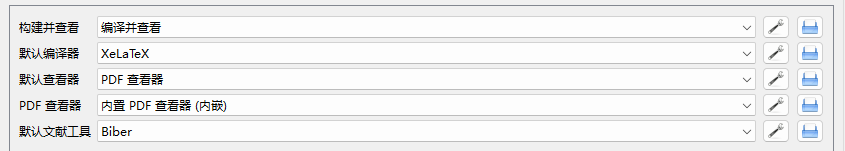
\includegraphics[width=\linewidth]{set.png}
		\caption{设置}
	\end{minipage}
\end{figure}

   \end{spacing}
   \clearpage
\fancyhf{} % 清空页眉和页脚
\fancyfoot[C]{\thepage} % 设置页脚中间显示页码
\renewcommand{\headrulewidth}{0pt} % 去除页眉线
\printbibliography[title={参考文献}]

   \pagenumbering{Roman} % 设置页面编号为大写罗马数字
   \setcounter{page}{\value{romanpage}}  % 设置页码继续摘要后的罗马数字页码
   \clearpage
\fancyhead{} % 将页眉设置为空

\vspace*{24pt}
\centerline{\Large\rmfamily\bfseries 致\quad 谢}
\addcontentsline{toc}{chapter}{\protect\numberline{致\quad 谢}{}}
\vspace*{18pt}
\fontsize{12}{20}\selectfont}

欢迎使用本模板,使用过程中出现什么问题可以与ligy1920@mails.jlu.edu.cn联系.
\end{document}
